\setchapterstyle{kao}
\setchapterpreamble[u]{\margintoc}
\chapter{AT2019dsg}
\labch{intro}

On 2019 October 1, the IceCube Neutrino Observatory reported the detection of a $\sim$0.2 PeV neutrino, IC191001A, with a 59\% probability of being of astrophysical origin \cite{stein:gcn25913} (see Chapter \ref{ch:realtime}). Seven hours later, the direction of the incoming neutrino was observed by ZTF as part of our neutrino follow-up program. The data was processed by our multi-messenger pipeline (see Chapter \ref{ch:ztf_too}) and the radio-emitting tidal disruption event AT2019dsg was identified as a candidate neutrino source \cite{2019ATel13160....1S}.

\section{Discovery of AT2019dsg}

AT2019dsg was discovered by ZTF on 2019 April 9 under the name \emph{ZTF19aapreis}, and reported on 2019 April 22 as a likely extragalactic transient by AMPEL \sidecite{2019TNSTR.615....1N}. AT2019dsg was publically classified as a TDE on 2019 May 13 by ePESSTO+ on the basis of its optical spectrum\sidecite{2019ATel12752....1N}.  All candidate TDEs identified by ZTF are named after characters from HBO series \emph{Game of Thrones}. As the nth candidate TDE, AT2019dsg was given the official nickname of \emph{ZTF-BranStark} \sidecite{2020arXiv200101409V}. 

Radio emission was tentatively reported on 2019 May 23 by AMI-LA \cite{2019ATel12798....1S}, and confirmed on 2019 July 26 by e-MERLIN \cite{2019ATel12960....1P}. The potential neutrino association was reported on 2019 October 2 \sidecite{2019ATel13160....1S}. In addition to observations as part of a systematic ZTF search for TDEs \cite{2020arXiv200101409V}, the association with IC191001A prompted additional follow-up. 

\section{Observation of AT2019dsg}

\begin{figure}[!ht]
	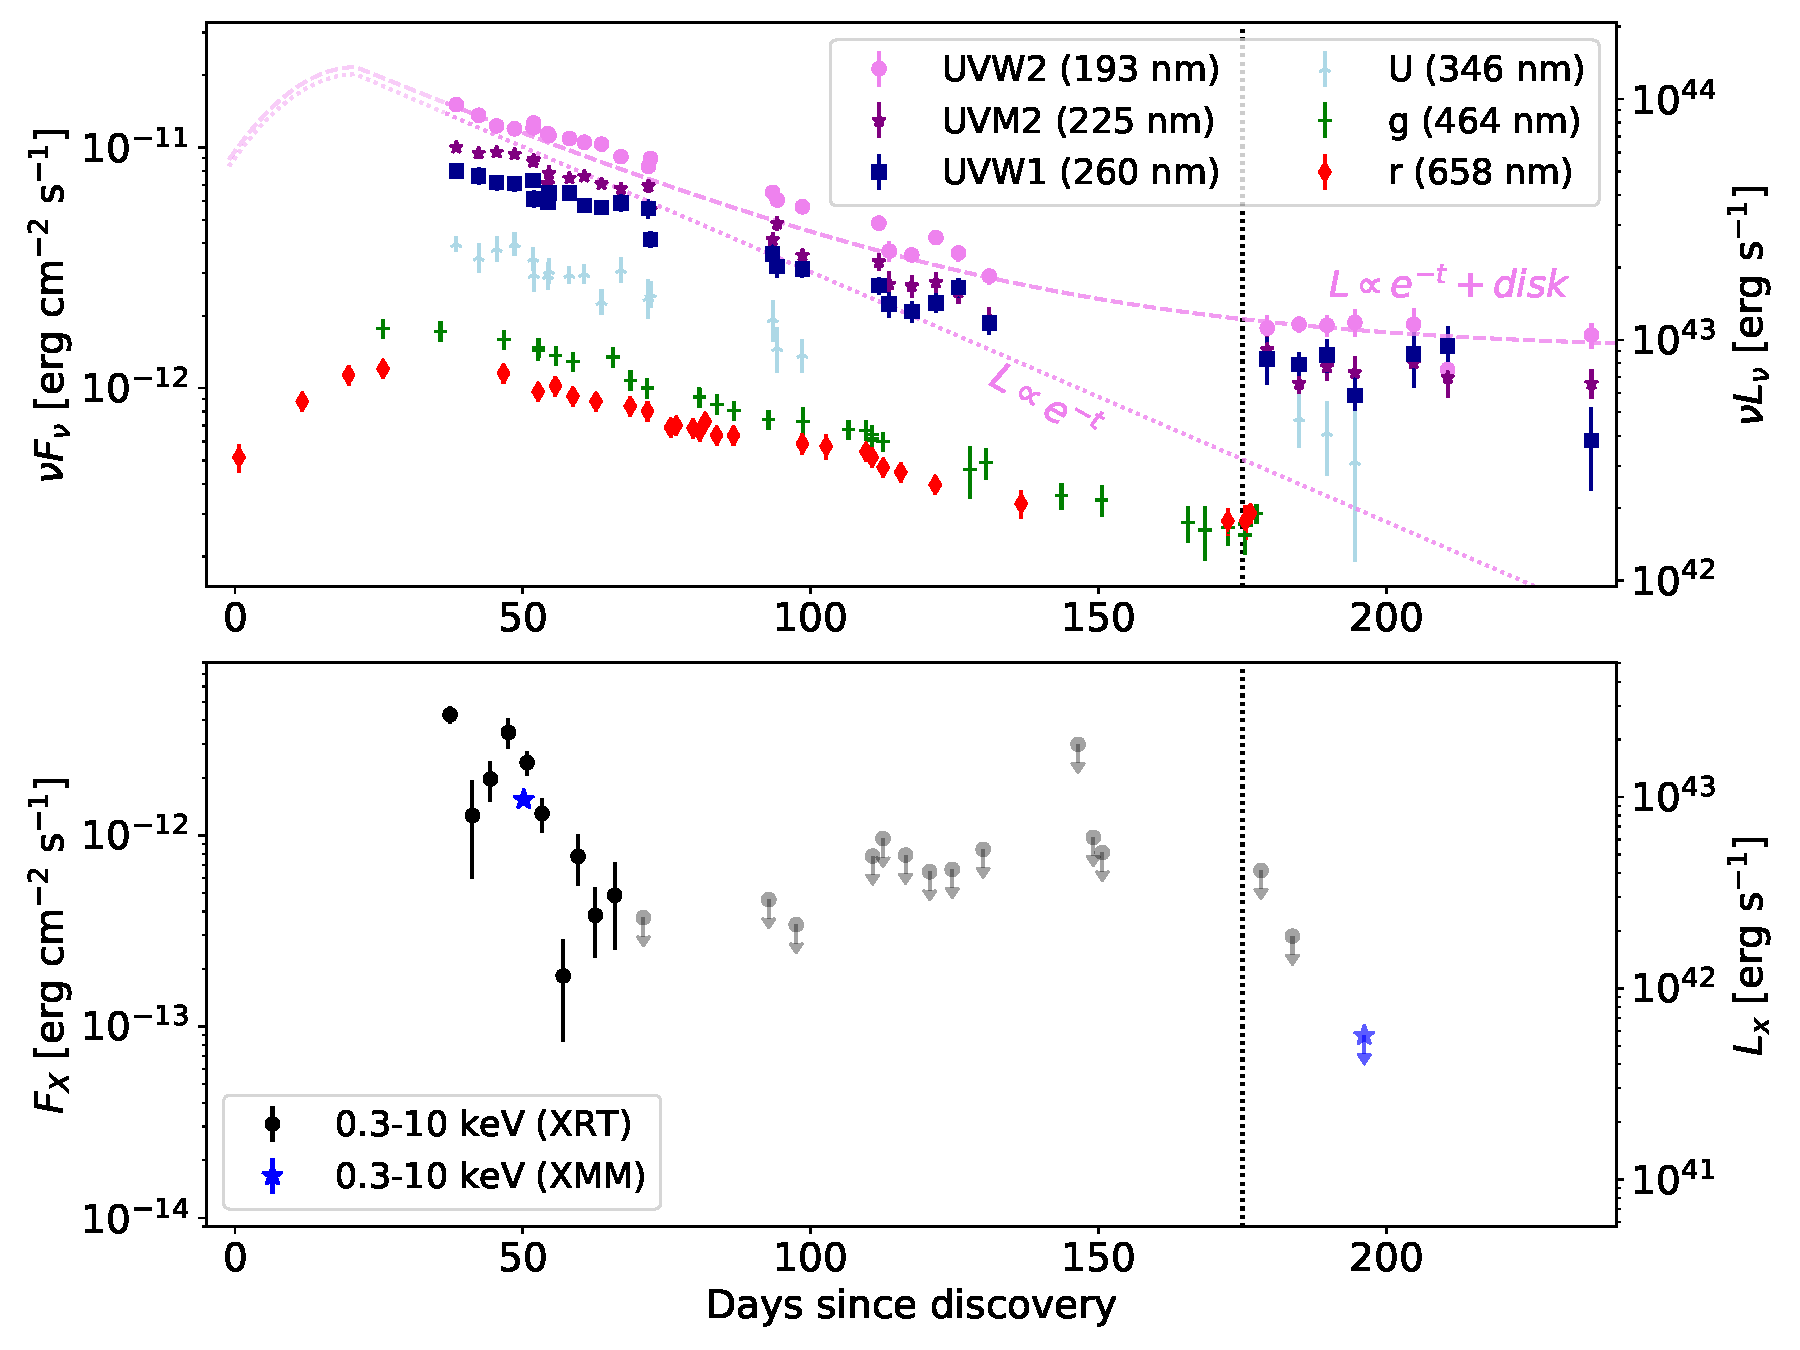
\includegraphics{Bran/lightcurve_wfit.pdf}
	\caption{Multi-wavelength lightcurve of AT2019dsg. Error bars represent 1$\sigma$ intervals. The upper panel shows the optical photometry from ZTF, alongside UV observations from \textit{Swift}-UVOT. The plateau luminosity is a factor of 10 brighter in UVW2 than the pre-disruption baseline of the host galaxy. The lower panel shows the integrated X-ray energy flux, from observations with \textit{Swift}-XRT and \textit{XMM-Newton}, in the energy range 0.3-10 keV. Arrows indicated 3$\sigma$ upper limits.  The vertical dotted line illustrates the arrival of IC191001A.}
	\label{fig:bran_lightcurve}
\end{figure}

\subsection{Optical/UV}

 The optical/UV continuum of AT2019dsg is well described by a single blackbody photosphere with a near-constant temperature \cite{2020arXiv200101409V} of $10^{4.59 \pm 0.02}$~K and radius of $10^{14.59 \pm 0.03}$~cm. The peak luminosity of $10^{44.54 \pm 0.08}$ erg\,s$^{-1}$ is in the top 10\% of the 40 known optical TDEs to date \cite{2020arXiv200101409V}, and the temperature is in the top 5\%. By the time of the neutrino detection, the optical/UV luminosity appeared to have reached a plateau (see Figure \ref{fig:bran_lightcurve}). Such plateaus are common in TDEs and interpreted as emission from the outer part of an accretion disk \cite{2019ApJ...878...82V,2020MNRAS.492.5655M}, but typically occur a few years after peak. The rapid appearance of an accretion-disk plateau would be expected for disruptions around higher-mass SMBHs. Indeed the total mass of the host galaxy of AT2019dsg is in the top 10$\%$ of all optical TDE hosts. Assuming 50$\%$ of the host mass is in the bulge, we estimate \cite{2013ApJ...764..184M} a black
hole mass of $\sim 3 \times 10^{7} \Msol$.

Prior to the detection of IC191001A, AT2019dsg had already been repeatedly detected by ZTF P48 telescope as part of the public MSIP survey, most recently on 2019 September 28. These data were supplemented by photometric observations from the 2m Liverpool Telescope\cite{2004SPIE.5489..679S} and SEDM\cite{Blagorodnova18,Rigault19} photometry\cite{fst+2016} obtained using the P60 telescope on Mt Palomar. ToO observations of the neutrino localisation field began on 2019 October 1, 7.4 hours after the neutrino detection. A second set of observations were performed the following night. In all of these images AT2019dsg was clearly visible. 

UV observations of AT2019dsg were conducted as part of a systematic survey of UV properties of all ZTF-identified TDEs\cite{2018ApJ...852...72V}, using the UltraViolet/Optical Telescope\cite{2005SSRv..120...95R} (UVOT) on board the \textit{Neil Gehrels Swift Observatory} (\textit{Swift})\cite{2004ApJ...611.1005G}. Data were reduced with \texttt{uvotsource} using an aperture of 7" to capture the entire galaxy (the host flux density was subtracted based on the best-fit galaxy model\cite{2018ApJ...852...72V} and uncertainties on this baseline are propagated into the reported UVOT difference photometry). The first UV observation was performed 15 days after the optical peak on 2019 May 17, and a bright source spatially coincident with the TDE was detected. Subsequent observations continued at a cadence of 2--3 days, up to 2019 September 7. In this period, AT2019dsg continued to steadily dim. An additional observation occurred shortly before the neutrino detection on 2019 September 27. Follow-up observations were then triggered by the identification of a possible association with IC191001A\cite{2019ATel13160....1S}, beginning on 2019 October 5. 

The optical/UV data are summarised in Table \ref{tab:photometry}. We note that in the final ZTF observations, the source appears to redden in the optical bands. This could be a signature of reverberation due emission from dust heated by the TDE\cite{2016ApJ...829...19V,2016MNRAS.458..575L}; this dust can reach a temperature of $\sim 2000$ K. An important caveat is that the contrast between the transient emission and the host is very small for these late-time optical detections, so the residuals in the difference image may need to be corrected to account for small systematic offsets. That can only be investigated when the images for this portion of the public survey are published as part of the next ZTF data release. We note that the UV observations are not subject to the same uncertainty because even at late times the transient UV flux is about an order of magnitude brighter than the host baseline.

\subsection{X-ray}

AT2019dsg was also detected in X-rays, beginning 37 days after discovery. Though the first X-ray observation indicated a bright source, with a high X-ray to optical ratio of $L_{\textup{X}}/L_{\textup{opt}} \sim $0.1, this X-ray flux faded extremely rapidly, as shown in Figure \ref{fig:bran_lightcurve}. This rate of decline is unprecedented, with at least a factor of 50 decrease in X-ray flux over a period of 159 days. Similar to the optical/UV emission, the observed X-ray spectrum is consistent with thermal emission, but from a blackbody of temperature $10^{5.9}$ K ($0.072 \pm 0.005$ keV) and, assuming emission from a circular disk, a radius $\sim 2 \times 10^{11}$ cm. As for most X-ray-detected TDEs\cite{2017ApJ...838..149A, 2019MNRAS.487.4136W,2019ApJ...872..198V}, the blackbody radius appears much smaller than the Schwarzschild radius ($R_{\textup{S}} \sim 10^{13}$~cm) inferred from the galaxy scaling relation\cite{2013ApJ...764..184M}. Small emitting areas can arise from an edge-on orientation, because the relativistic velocities at the inner disk can Doppler boost a large area of the disk out of the X-ray band.  Since our observations probe close to the Wien tail of the spectrum, a small temperature decrease due to absorption would also yield a significantly underestimated blackbody radius and luminosity\cite{2019ApJ...872..198V}. The exponential decrease of the flux could be caused by cooling of the newly-formed TDE accretion disk\cite{2020MNRAS.492.5655M} or increasing X-ray obscuration.

AT2019dsg was first observed in X-rays on 2019 May 17 by the X-Ray Telescope (XRT)\cite{2005SSRv..120..165B}, also on board \textit{Swift}\cite{2004ApJ...611.1005G}, as part of a program to categorise the X-ray properties of TDEs. AT2019dsg was detected at high significance at this epoch, with a measured energy flux of $F_{X}\sim 4 \times 10^{-12}$ erg cm$^{-2}$ (0.3--10 keV). Observations continued with a cadence of 2--3 days, and indicated a sharply-declining X-ray flux. The source was last detected on 2019 June 14, and not detected again in any of the following observations continuing until 2019 September 7. An additional observation was performed with the \textit{X-ray Multi-Mirror Mission} (\textit{XMM-Newton}) telescope on 2019 May 30, in the range 0.3-10 keV. The \textit{XMM-Newton} EPIC-pn observations (programs 082204 and 08425; P.I. Gezari) were taken in Wide window Thin1 filter mode and reduced using standard techniques with the \textit{XMM-Newton}\cite{2001A&A...365L...1J} Science Analysis System (SAS). The source extraction region was a circle of radius 35 arcsec at the location of the optical transient in the X-ray image, and the background was measured using a 108-arcsec circular region (shown in Figure \ref{fig:xraymap}). The \textit{XMM} spectrum was binned using the \texttt{GRPPHA} command, such that there were at least 20 counts contained in each bin. It was then fit ($\chi^2/\textup{dof}=59.26/65$) with the  disk blackbody (\texttt{diskbb}) model with Galactic\cite{HI4PI2016} and intrinsic ($N_{\textup{H}} \sim 4 \times 10^{20}$ cm$^{-2}$) absorption described using the \texttt{phabs} model in \texttt{XSPEC} v12.9.1\cite{1996ASPC..101...17A}. The flux was consistent with those of \textit{Swift}-XRT, and provided a high signal-to-noise X-ray spectrum well-fitted with a single disk temperature of $T_{\textup{disk}} = 10^{5.9}$ K (0.072 $\pm 0.005$ keV), shown in Figure \ref{fig:xrayspec}. Following the identification of AT2019dsg as a candidate counterpart to IC191001A\cite{2019ATel13160....1S}, additional X-ray observations were triggered. AT2019dsg was again not detected, with the first \textit{Swift}-XRT observation occurring on 2019 October 5. An additional \textit{XMM} observation on 2019 October 23 yielded a deep upper limit of $9 \times 10^{-14}$ erg cm$^{-2}$ s$^{-1}$ (0.3--10 keV) using the same thermal model, computed at the 3$\sigma$ confidence level using the \textit{XMM} SAS/HEASARC command \texttt{eregionanalyse}. 

\begin{marginfigure}
	\centering
	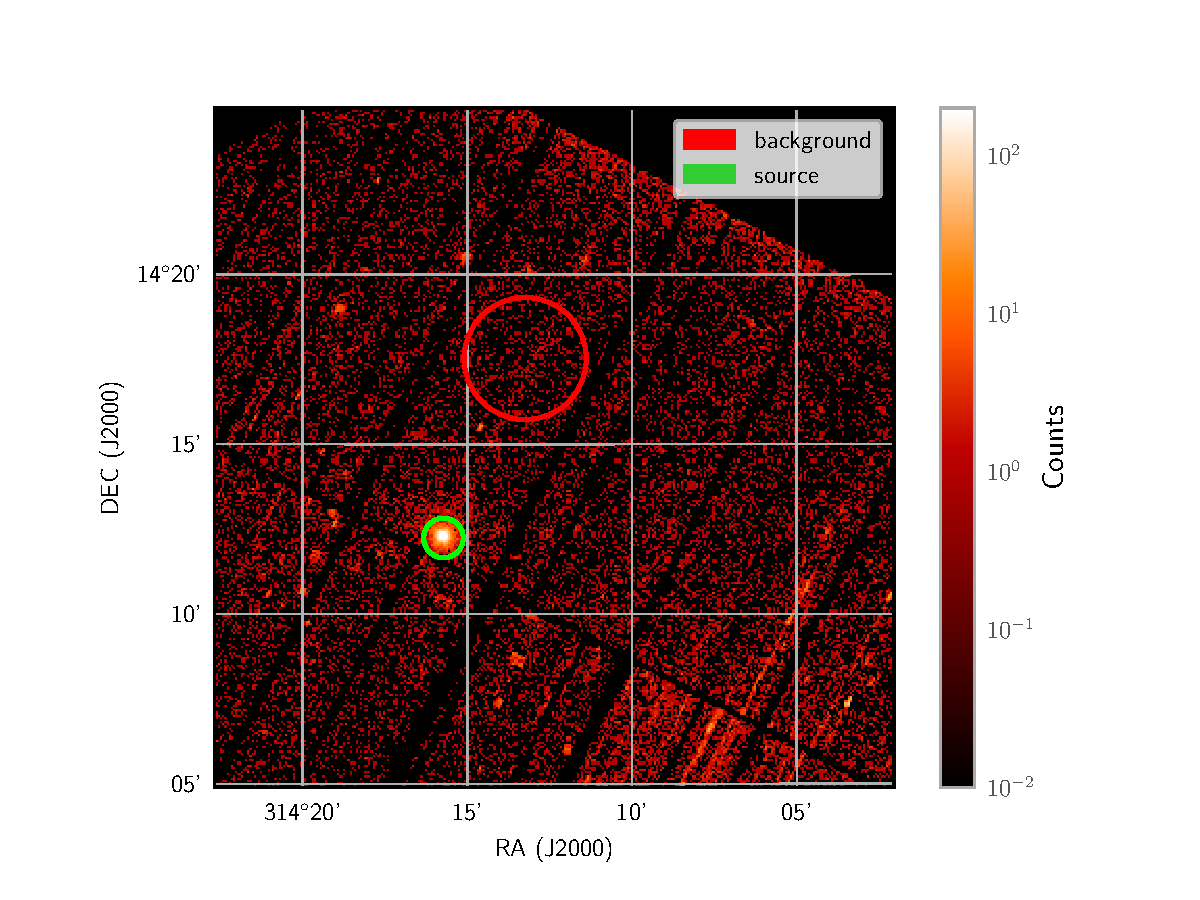
\includegraphics{Bran/Bran_XMM_epoch1_region.pdf}
	\caption{X-ray count map from \textit{XMM-Newton} (50 days after discovery). The green circle indicates the source region, while the red circular region was used to measure the background. The best-fit position derived from optical observations is spatially-coincident with the center of the X-ray source region.}
	\label{fig:xraymap}
\end{marginfigure}

\begin{figure*}
	\centering
	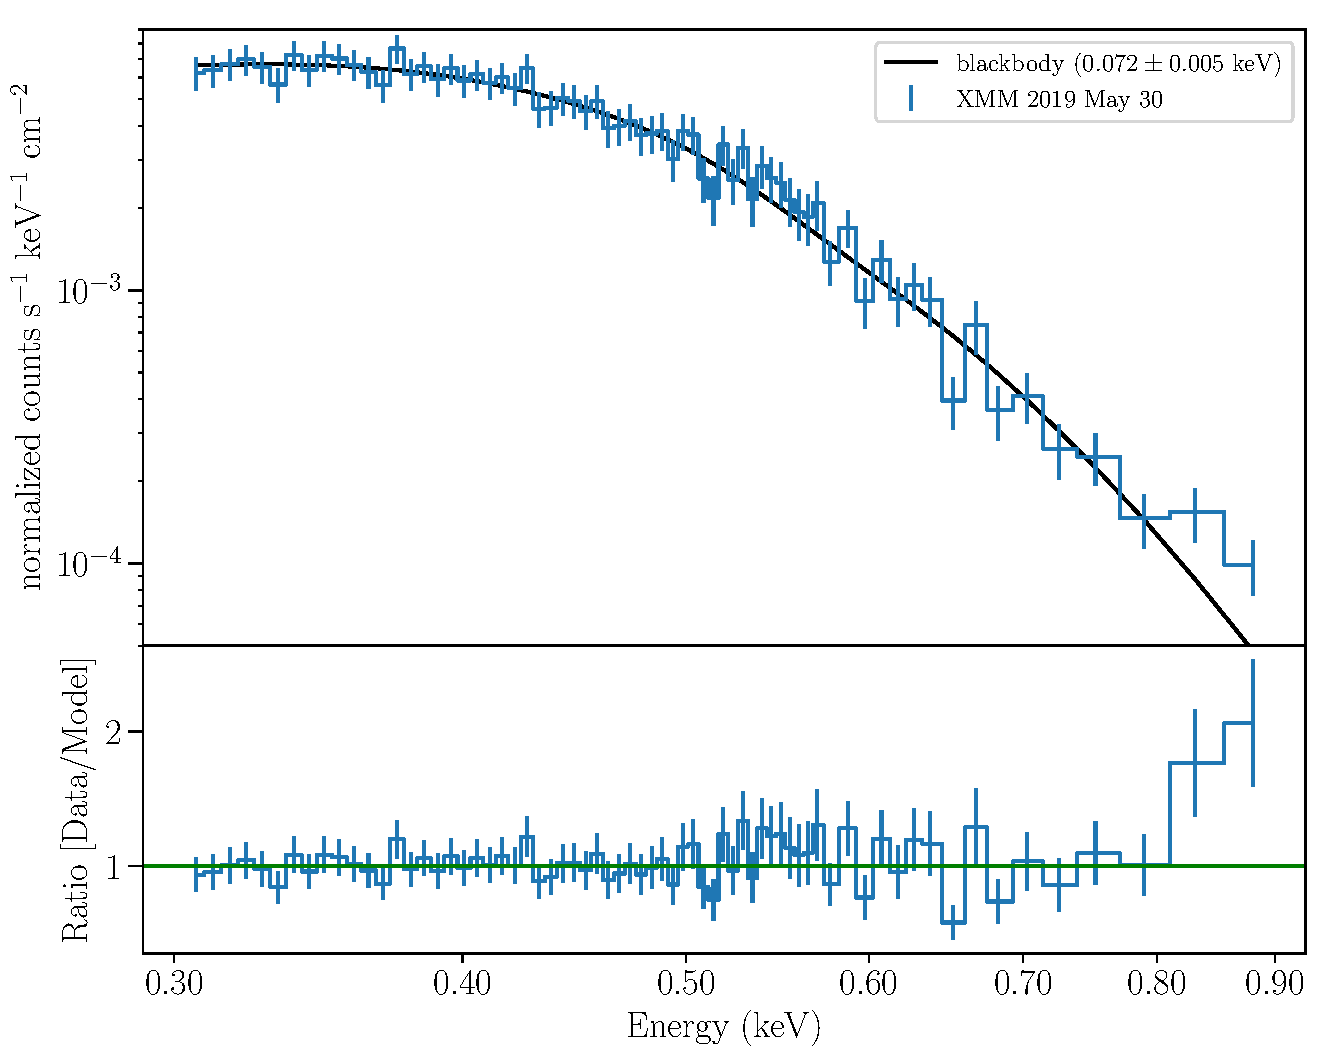
\includegraphics[width=0.95\textwidth]{Bran/3eyedraven_xmm_spc_0842590901_abs.pdf}
	\caption{Soft X-ray spectrum of AT2019dsg measured by \textit{XMM-Newton}, fitted with an absorbed disk blackbody model. Error bars represent 1$\sigma$ intervals.}
	\label{fig:xrayspec}
\end{figure*}

\subsection{Radio}

Radio observations shown in Figure \ref{fig:radio_spectrum} reveal a third distinct spectral component, namely synchrotron emission from non-thermal electrons. We model this emission with a  conical geometry as expected for outflows (e.g., jets or winds) that are launched from---and collimated by---the inner parts of flared accretion disks that emit close to the Eddington limit.
Given that electrons are typically accelerated with much lower efficiency than protons in astrophysical accelerators\cite{2012A&A...538A..81M}, we assume that they carry 10\% of the energy carried by relativistic protons ($\epsilon_{e} = 0.1$). We further assume that the magnetic fields carry 0.1\% of the total energy ($\epsilon_{B} = 10^{-3}$), as indicated by radio observations of other TDEs\cite{2018ApJ...854...86E} and supernovae\cite{2013MNRAS.436.1258H}. For a half-opening angle, $\phi$, of 30\arcdeg\ we find $R = 1.5 \times 10^{16}$ cm in our first epoch (41 days after discovery), increasing to $R = 7 \times 10^{16}$~cm shortly after the neutrino detection (177 days after discovery).  These radii scale\cite{2013ApJ...772...78B} as $R \propto [1-\cos(\phi$)]$^{-8/19}$. The implied expansion velocity is roughly constant at $v/c = \dot{R}/c = 0.12 \pm 0.01 $ during the first three epochs, with an acceleration to $v/c = 0.21 \pm0.02$ for the last epoch.  These are the velocities of the synchrotron-emitting region, and thus provide a lower limit to the velocity at the base of the outflow.  Indeed even the hotspots of relativistic jets from active galaxies that are frustrated by gas in their host galaxy are typical observed\cite{2003PASA...20...69P} to have subrelativistic expansion velocities of $\sim0.1c$. 

The inferred outflow energy, $E$, shows a linear increase from $2.5 \times 10^{49}$~erg to $2 \times 10^{50}$~erg (Figure \ref{fig:radio_spectrum}), which is not expected in models\cite{2016ApJ...819L..25A,2016ApJ...827..127K} of TDE radio emission that involve a single injection of energy. While some scenarios can yield an increase in inferred energy from a single energy injection, none of these are consistent with the full set of observed properties. First, a single ejection with a range of velocities could explain the observed linear increase of energy with time (the slower ejecta arrive later), but is incompatible with the increasing velocity. Second, an increase of the efficiency for conversion of Poynting luminosity to relativistic particles is unlikely because the target density that is available to establish this conversion is decreasing.  And finally, an increase of solid angle that emits to our line of sight is only expected for relativistic outflows that decelerate. Instead, for AT2019dsg, the observations suggest the presence of a central engine that yields continuous energy injection through a coupling of accretion power to the radio emission\cite{2018ApJ...856....1P}, with acceleration in the final radio epoch due to a decrease in the slope of the ambient matter density profile. 

Four observations of AT2019dsg were performed with the Karl G.\ Jansky Very Large Array (VLA) under project code 19A-395 (PI: van~Velzen), on 2019 May 22, June 19, August 8 and October 5.  The array was in its moderately-extended B configuration (maximum baseline 11\,km) for the first two epochs, and in its most extended A-configuration (maximum baseline 36\,km) for the final two epochs.  Our first epoch, on May 22, was a detection experiment, and we observed only in the 8--12\,GHz band.  Having established the presence of radio emission, we observed over a broader range of frequencies in the subsequent three epochs, using the 2--4\,GHz, 4--8\,GHz, and 8--12\,GHz bands.  We used 3C\,48 as a bandpass and flux density calibrator on May 22, and 3C\,286 for the other three epochs.  We used the nearby extragalactic sources ICRF J204945.8+100314 
% MFB: we should give source names that resolve on e.g. Simbad, and good to mention its an ICRF source - our posn accuracy should be good.
(at 4--8 and 8--12\,GHz) and ICRF J203533.9+185705 (at 2--4\,GHz) to determine the complex gain solutions, which were interpolated to AT2019dsg. We used the Common Astronomy Software Application (CASA)\cite{McMullin2007} Calibration pipeline (v5.4.1) to perform external gain calibration, and after removing residual radio frequency interference, we imaged the data within CASA, using Briggs weighting with a robust parameter of 1.  We split each baseband into multiple frequency bins for imaging (1\,GHz bins above 4\,GHz, and 0.5\,GHz bins below that) to provide better sampling of the broadband spectrum, allowing more precise constraints on the turnover frequency, and better spectral modelling.

% two paragraphs from AMI 
Radio observations of the field of AT2019dsg were also conducted using the AMI Large Array (AMI-LA)\cite{2008MNRAS.391.1545Z,2018MNRAS.475.5677H}. AMI-LA is a radio interferometer comprised of eight 12.8m-diameter antennas producing 28 baselines that range from 18m up to 110m, which operates with a 5 GHz bandwidth around a central frequency of 15.5 GHz. We observed AT2019dsg on several epochs (see Table \ref{tab:radio_data}) for four hours each. Initial data reduction, editing, and calibration of the phase, and flux density, was carried out using \verb reduce_dc , a customized AMI data reduction software package\cite{2015MNRAS.453.1396P}. Phase calibration was conducted using short interleaved observations of ICRF J205135.5+174336,
%MFB was: J2051+1743, 
while for absolute flux density calibration we used 3C\,286. Additional flagging and imaging were performed using CASA. All of our observations showed a source consistent with the location of AT2019dsg. We used the CASA task IMFIT to find the source flux and position. 

Further observations of AT2019dsg were conducted with the South African MeerKAT telescope, on 2019 June 19, July 29, October  5, and November 30, with each session being $\sim$2~h long.  We used ICRF J193925.0-634245 as a flux-density calibrator, and ICRF J213032.8+050217 as a phase and amplitude calibrator.  The initial calibration was done using the IDIA MeerKAT pipeline\footnote{\url{https://idia-pipelines.github.io/docs/processMeerKAT}}, which is implemented in CASA\@.  The observed band was 860 MHz wide and centred on 1280 MHz. We imaged the whole primary beam ($\sim 1$\arcdeg) using the CLEAN algorithm (CASA: tclean) in order to remove sidelobes from the many (unrelated) sources within the primary beam.  The total CLEAN flux density in the field was $\sim$1~Jy, and the peak brightness in the images was about 48 mJy~beam$^{-1}$ (not related to AT2019dsg). Since residual small calibration errors dominated the image rms background in the initial images, we self-calibrated the data in both phase and amplitude, with the mean amplitude gain being fixed at unity to minimise any drifting of the flux-density scale. The resolution is slightly different in each epoch, but was $\sim$11\arcsec\ north-south, and $\sim$6\arcsec\ east-west.  Image rms background levels also varied, ranging between 25 and 32 $\mu$Jy~beam$^{-1}$.  There was no sign of extended emission or confusing sources near AT2019dsg. The flux density was determined by fitting an elliptical Gaussian with the same geometry as the restoring beam to the images.  

The measured flux densities from our radio observations are reported in Table \ref{tab:radio_data}. For all radio observations, the reported uncertainties include both the image background rms and a 5\% fractional calibration uncertainty, added in quadrature.

\subsection{Gamma-ray}

We analysed data from the %pair-conversion telescope 
\textit{Fermi} Large Area Telescope (\textit{Fermi}-LAT)\cite{2009ApJ...697.1071A}, sensitive to gamma rays with energies from 20 MeV to greater than 300 GeV. During its sky-survey operations, the pair-conversion telescope \textit{Fermi}-LAT scans the entire sky about every three hours, and can monitor the variable gamma-ray sky over short and long timescales. We studied the region of AT2019dsg in three different time intervals, motivated by the multi-wavelength behavior of the source. The first interval (G1) includes 130 days of observations that include the peak of the optical emission from 2019 April 4 to 2019 August 12. The second one (G2) spans 2019 August 12 to 2019 November 20 and covers the UV plateau and the peak of the radio emission. The third period (G3) integrates the whole period between the start of G1 up to 2020 January 31. We use the photon event class from Pass 8 \textit{Fermi}-LAT data (P8R3\_SOURCE), and select a $15\arcdeg \times 15\arcdeg$ Region of Interest (RoI) centered on the AT2019dsg position derived from optical observations, with photon energies from 100 MeV to 800 GeV. We use the corresponding LAT instrument response functions P8R3\_SOURCE\_V2 with the recommended spectral models \textit{gll\_iem\_v07.fits} and \textit{iso\_P8R3\_SOURCE\_V2\_v1.txt} for the Galactic diffuse and isotropic component respectively. To minimise contamination from gamma rays produced in the Earth's upper atmosphere, we require an instrumental zenith angle $\theta<90\arcdeg$ for all events, in addition to the standard data quality cuts suggested by the \textit{Fermi} Science Support Center\footnote{\url{https://fermi.gsfc.nasa.gov/ssc/data/analysis/scitools/data_preparation.html}}. We perform a likelihood analysis, binned spatially with $0.1 \arcdeg$ resolution and 10 logarithmically-spaced bins per energy decade, using the \textit{Fermi}-LAT ScienceTools package (fermitools v1.0.1) along with the \textit{fermipy} package v0.17.4\cite{2017ICRC...35..824W}.

A search was already performed within the 90\%\ error region during both the 1-day and 1-month period prior to the arrival of the high-energy neutrino\cite{garrappa_buson:gcn25932}. No new gamma-ray source was identified, and there was no significant ($\geq 5 \sigma$) detection for any source from the fourth \textit{Fermi}-LAT point source catalog (4FGL\cite{2019arXiv190210045T}). Here, we specifically test a point-source hypothesis at the position of AT2019dsg under the assumption of a power-law spectrum. We find TS\footnote{TS is twice the difference in the maximum $\log \mathcal{L}$ of an ROI model with and without the source, where $\mathcal{L}$ is the likelihood of the data given the model.} = 0 for all intervals. Upper limits for the energy flux (integrated over the whole analysis energy range) have been derived for a power-law spectrum ($dN/dE \propto E^{-\Gamma}$) with photon power-law index $\Gamma$ = 2 and are listed in Table \ref{tab:lat_uls} along with the respective time intervals.

In all three time intervals, we detect a new, non-catalogued gamma-ray emitter in the RoI at a significance $\geq 5 \sigma$. This source lies just outside the IC191001A 90$\%$ error region, as indicated in Figure \ref{fig:fermi}. The source, which we label \textit{Fermi}-J2113.8+1120, is likely the gamma-ray counterpart of the radio-loud object GB6 J2113+1121, classified as a flat-spectrum radio quasar with redshift $z = 1.63$\cite{2013ApJ...767...14P}. The detection of an unrelated gamma-ray blazar within the neutrino uncertainty area is consistent with the background estimation. On average 1.5 4FGL gamma-ray blazars are expected in 20 sq.\,deg. In addition, a lightcurve analysis (Figure \ref{fig:fermi_lc}) reveals that the source is not significantly detected in gamma rays when IC191001A was detected. The lag between the closest significant detection of the source and the neutrino arrival was approximately $\sim$1 month. Such a lag is disfavored by recent studies on the temporal behavior of hadronic processes in blazars\cite{2015ApJ...802..133D,2019NatAs...3...88G}, suggesting that the blazar is unlikely producing the neutrino. %for which a shared origin of GeV photons and high-energy neutrinos from the same processes is disfavoured by recent studies on the temporal behavior of hadronic processes in blazars\cite{2015ApJ...802..133D,2019NatAs...3...88G}. 
Hence, given the lack of any obvious connection between the gamma-ray observations of \textit{Fermi}-J2113.8+1120 and IC191001A, we do not discuss this source any further.

The HAWC observatory also reported a search for transient gamma-ray emission on short timescales in the localisation of IC191001A\cite{ayala:gcn25936}, and set a limit for their most significant position at 95\% confidence of $E^{2} dN/dE = 3.51 \times 10^{-13} (\textup{E}/\textup{TeV})^{-0.3}$ TeV cm$^{-2}$ s$^{-1}$, in the energy range 300 GeV to 100 TeV, for the period from 2019 September 30 05:46:52 UTC to 2019 October 02 06:03:29 UTC. We note that this search covered a relatively large region of the sky, and thus had a large associated trial factor. A dedicated search at the position of AT2019dsg would be more sensitive, especially one that additionally targeted the longer period over which the central engine is active.

\begin{table}
	\centering
	\begin{tabular}{||c c c c||} 
		\hline
		\textbf{Interval} & \textbf{MJD Start} & \textbf{MJD Stop} & \textbf{UL}\\
		& & &  (erg cm$^{-2}$ s$^{-1}$)\\
		\hline
		\textit{G1} & 58577 & 58707 & 2.6 $\times 10^{-12}$\\
		\textit{G2} & 58707 & 58807 & 1.2 $\times 10^{-11}$\\
		\textit{G3} & 58577 & 58879 & 2.0 $\times 10^{-12}$\\
		\hline
	\end{tabular}
	\caption{Gamma-ray energy flux upper-limits for a point-source with power-law index $\Gamma$=2.0 at the position of AT2019dsg integrated over the analysis energy range 0.1-800 GeV.}
	\label{tab:lat_uls}
\end{table}

\begin{figure}
	\centering
	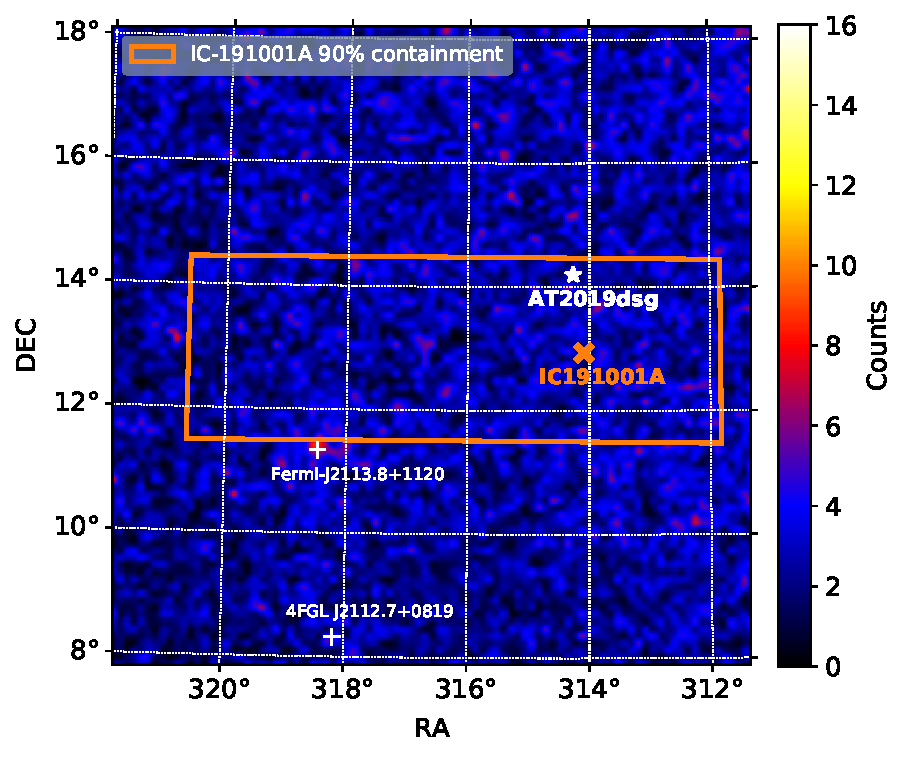
\includegraphics[width=\textwidth]{Bran/LAT_countsmap.pdf}
	\caption{LAT counts map of the Region Of Interest (ROI) in the integrated search period G3, showing the IC191001A 90$\%$ localisation region in green. The neutrino best-fit position is marked with a green `$\times$'. Two gamma-ray sources are significantly detected ($\geq$ 5 $\sigma$) in the ROI but outside the neutrino uncertainty region as marked with white crosses. There is no excess consistent with the position of AT2019dsg. %Gamma-ray sources significantly detected ($\geq$ 5 $\sigma$) are marked with white crosses. 
	}
	\label{fig:fermi}
\end{figure}

\begin{figure}
	\centering
	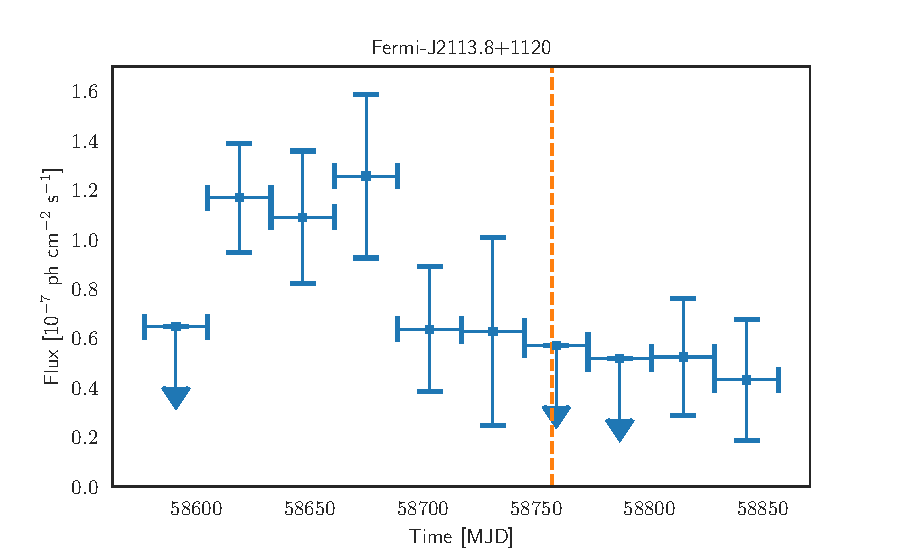
\includegraphics[width=0.8\textwidth]{Bran/fermi_lightcurve}
	\caption{LAT lightcurve in the 0.1-800 GeV energy range for the source \textit{Fermi}-J2113.8+1120 in the time interval G3, with evenly spaced binning of 28 days. Vertical error bars represent 1$\sigma$ intervals, horizontal bars denote bin width. 2$\sigma$ upper limits are shown for bins with TS$\leq$9. The orange dashed vertical line marks the arrival time of IC-191001A. Since this source lies outside the reported 90\% error region (see Figure~\ref{fig:fermi}), and given that the LAT lightcurve shows no obvious correlation with the neutrino arrival time, we conclude that it is unlikely to be associated with the neutrino.}
	\label{fig:fermi_lc}
\end{figure}


\subsection{Spectroscopy}


AT2019dsg was discovered by ZTF on 2019 April 9 under the name ZTF19aapreis, and publically reported as a  \sidecite{2019TNSTR.615....1N}, and was classified as a TDE on the basis of its optical spectrum\cite{2019ATel12752....1N} with a measured redshift of $z=0.051$, implying a luminosity distance $D_{\textup{L}} \approx$ 230 Mpc assuming a flat cosmology with $\Omega_{\Lambda}$ = 0.7 and $H_{0}$ = 70 km s$^{-1}$ Mpc$^{-1}$.

AT2019dsg was first classified as a TDE by ePESSTO+ on on 2019 May 13\cite{2019ATel12752....1N}, and the redshift of AT2019dsg was measured to be $z=0.051$. Further high-resolution spectroscopic observations were conducted using the De Veny Spectrograph on the 4.3m Lowell Discovery Telescope (LDT, PI: Gezari), the Kast Double Spectrograph on the 3m Lick Observatory Shane Telescope (Lick, PI: Foley)\cite{Miller93}, and the Low Resolution Imaging Spectrograph on the 10m Keck Telescope (Keck, PI: Graham)\cite{Oke95}, with the most recent spectrum on 2019 September 25. These spectra confirm that AT2019dsg belongs to the common spectroscopic class of TDEs with Bowen fluorescence emission lines and broad H$\alpha$ emission lines\cite{2020arXiv200101409V}. We note that the Ca triplet is also clearly visible in our late-time spectra (rest-frame 8498 \AA, 8542\AA ~and 8662 \AA), so the SMBH mass could in principle be inferred more precisely using higher-resolution spectroscopy of this feature\cite{2005MNRAS.359..765G}. Following the identification of AT2019dsg as a candidate neutrino source, additional high-resolution spectra of the source were taken with the 200in Hale Telescope Double Spectrograph at Palomar Observatory (P200, PI: Kasliwal \& Kulkarni) on 2019 October 3 and again with  Lick on 2019 October 5 and 2019 October 29 (shown in Figure \ref{fig:bran_spectrum}). There is no evidence of any significant spectral evolution between these spectra and the most recent pre-neutrino spectrum from 2019 September 25, and the spectral evolution of AT2019dsg is consistent with that of other TDEs\cite{2020arXiv200101409V}. 

\begin{figure*}[h!]
	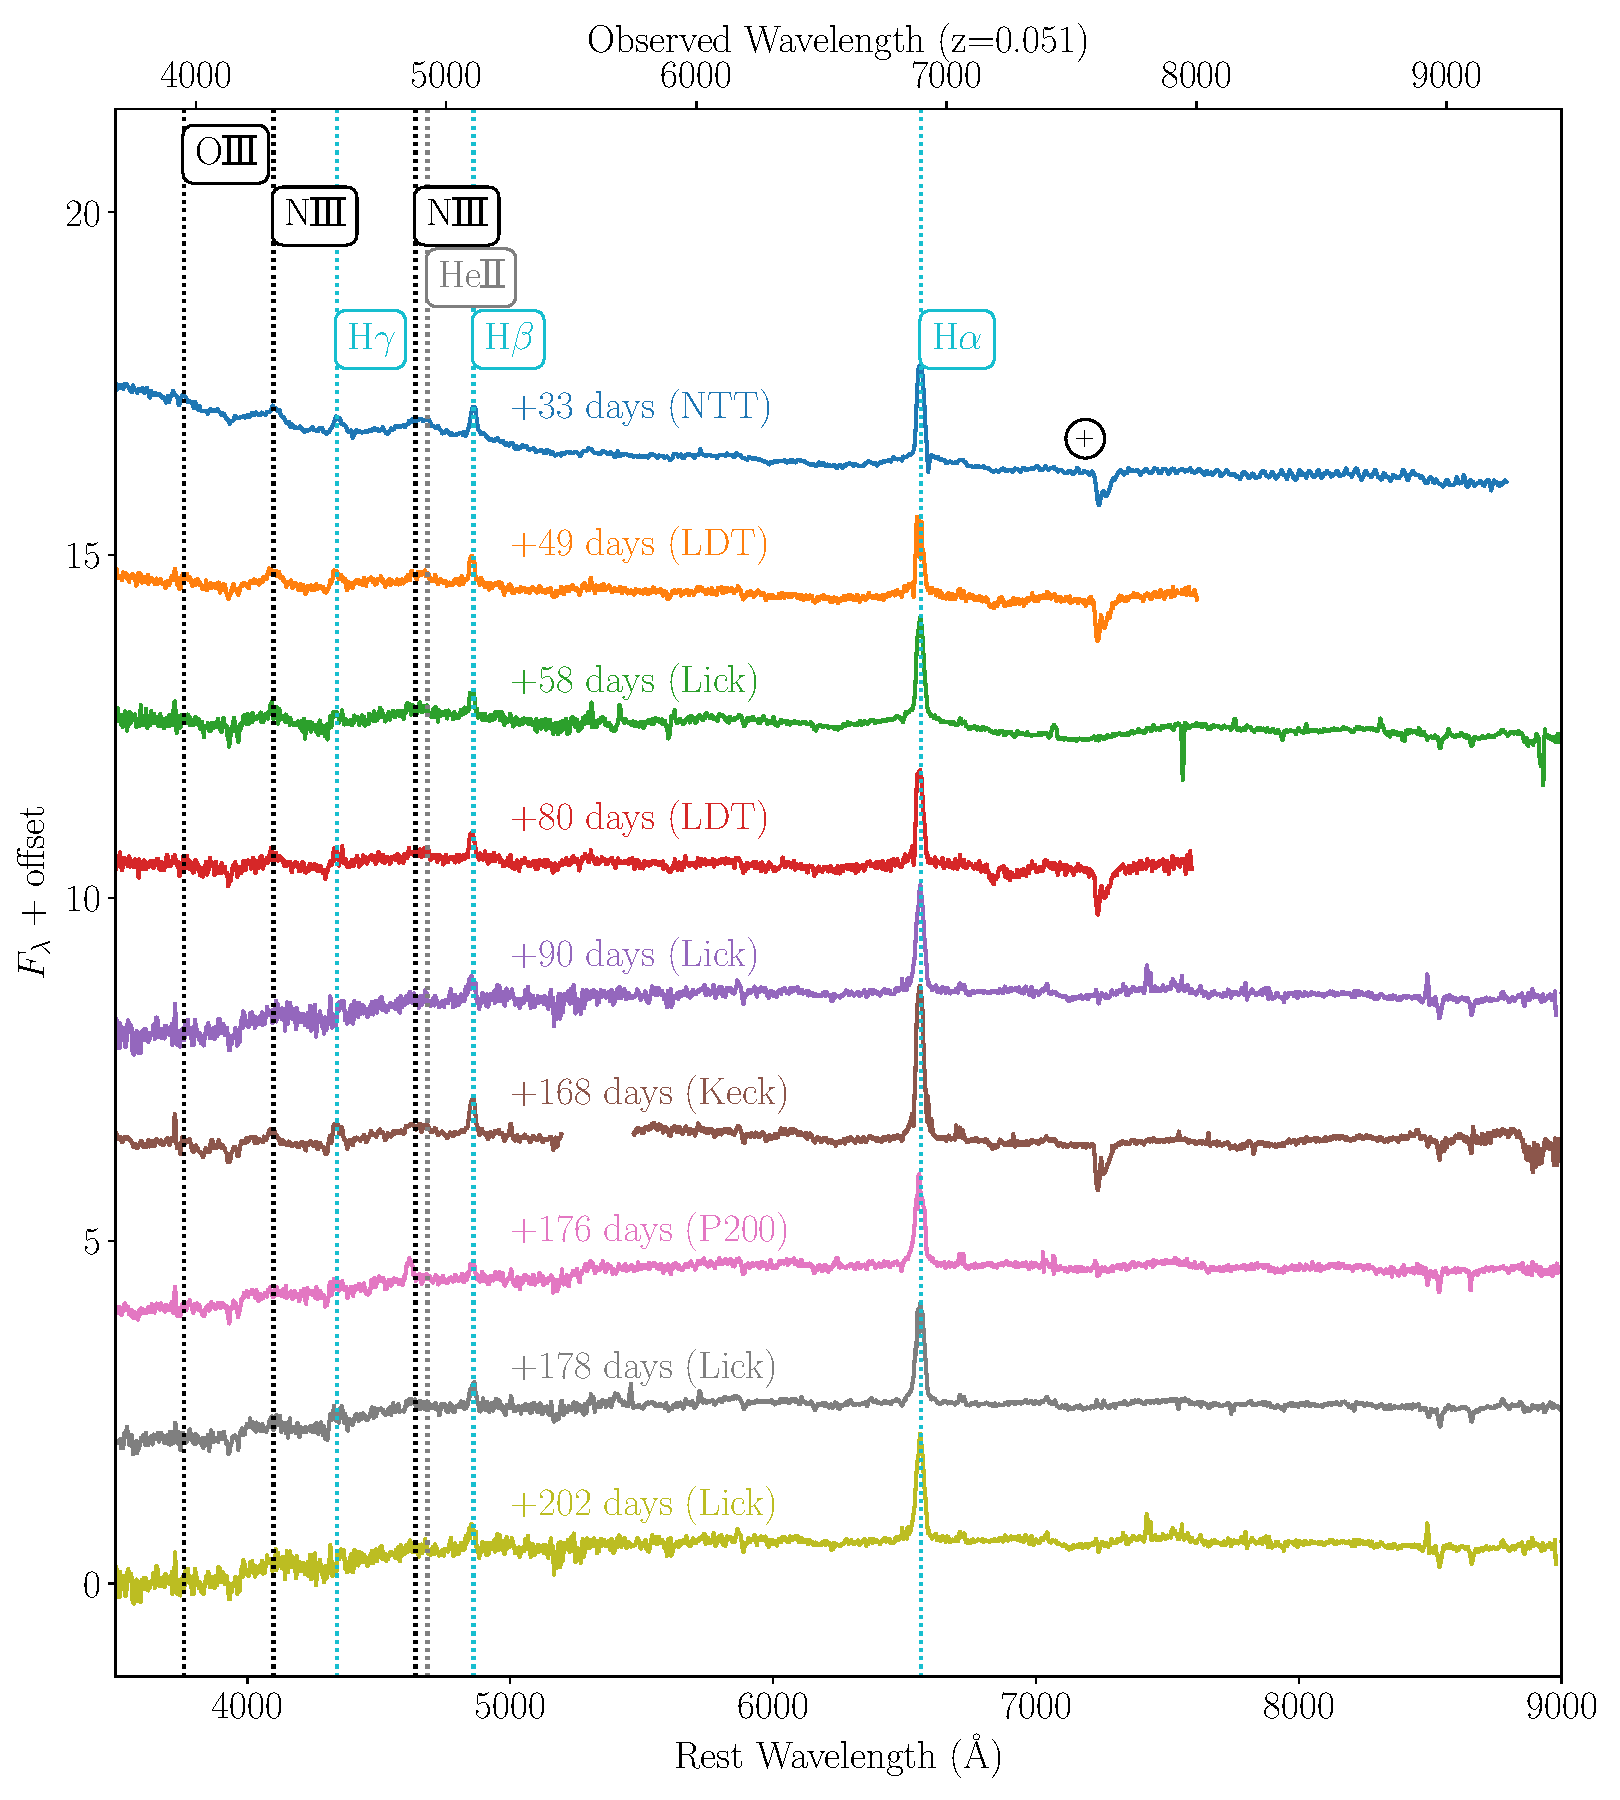
\includegraphics{Bran/spectra.pdf}
	\caption{The spectroscopic evolution of AT2019dsg, beginning with the publicly available classification spectrum taken with the NTT\cite{2019ATel12752....1N}, and further spectra from LDT, Lick, Keck and P200. The Balmer lines are highlighted in cyan, the HeII lines in gray, and the Bowen fluorescence lines (OIII at 3760\AA, NIII at 4100\AA ~and 4640\AA) in black. Telluric lines are marked with +.}
	\label{fig:bran_spectrum}
\end{figure*}

\section{Neutrino emission from AT2019dsg} With this strong evidence for three distinct emission zones derived purely from multi-wavelength observations, we consider whether this picture is consistent with AT2019dsg being the source of the neutrino IC191001A. In particular, neutrino production requires protons to be accelerated to sufficiently high energies, and to collide with a suitably abundant target. The detection of a single high-energy neutrino implies a mean expectation in the range $0.05 < N_{\nu, \textup{tot}} < 4.74$ at 90\% confidence, where $N_{\nu, \textup{tot}}$ is the cumulative neutrino expectation for all TDEs that ZTF has observed. AT2019dsg emits $f_{\textup{bol}} \sim 0.16$ of the population bolometric energy flux, and if we take this as a proxy for neutrino emission, we would expect $0.008 \lesssim N_{\nu} \lesssim 0.76$ for this source.

% Accounting for the large Eddington bias that arises from the Poisson-dominated emission of single high-energy neutrinos\cite{2019A&A...622L...9S}, the TDE should reasonably have sufficient flux to produce an expected number of high-energy neutrino alerts $N_{\nu} \sim$ 0.01-1. 

Radio observations confirm that particle acceleration is indeed occurring, and that this continues without decline through to the detection of the neutrino at $\sim$180 days post-discovery. Given that neutrinos typically take a fraction $\eta_{p\nu} \sim 0.05$ of the parent proton energy, our accelerator must be capable of accelerating protons to at least 4 PeV. We evaluate the Hillas criterion \sidecite{1984ARA&A..22..425H} that the proton Larmor radius be less than the system size, to determine whether this is possible. We use  our estimates for conditions in the synchrotron zone at the time of neutrino detection, with $B \sim$ 0.07 G and $R \sim 7 \times 10^{16}$ cm for the near-contemporaneous radio epoch. Taking this as a baseline, we find a maximum proton energy of $\sim$160 PeV, far in excess of our requirements. The Hillas criterion can also be satisfied within the engine that powers the radio-emitting outflow because the product $BR$ is not expected to decrease at smaller radii (e.g. $B \propto R^{-1}$ for a toroidal configuration). 

The target for neutrino production can be either photons (p$\gamma$ interactions) or protons (pp interactions). For a photon target, neutrino production occurs above an energy determined by the mass of the $\Delta$ resonance, $m_{\Delta}$. For a thermal spectrum, of temperature $T$, we then find $\epsilon_{\nu} \sim \eta_{p\nu}[(m_{\Delta}^{2} - m_{p}^{2})/ 4 \epsilon_\gamma ] \approx 0.3 \times \left(T/10^{5} \textup{K} \right)^{-1} \textup{PeV}$. For the UV photosphere of the TDE, we find $\epsilon_\nu \sim$ 0.8 PeV, while for the compact X-ray source, we find $\epsilon_\nu \sim$ 0.05 PeV. Both of these values are compatible with the observed neutrino, for which there is a typical uncertainty of one energy decade\cite{2018Sci...361.1378I}, so either photon field could serve as a target. For the UV photosphere, we find that the mean free path for the parent proton of a PeV neutrino ($\sim2 \times 10^{13}$ cm, see SI) is much smaller than the photosphere radius, so the UV photosphere is indeed optically thick. At smaller radii, the X-rays would overtake the UV photons as dominant scattering targets. 

In the multi-zone model shown in Figure \ref{fig:diagram}, the thermal photons provide a guaranteed target for pion production. However hadrons could in principle also serve as a target, leading us to consider a single-zone scenario in which the protons are accelerated at the same location as the synchrotron-emitting electrons, with the neutrino spectrum following the same intrinsic energy power law as the protons and electrons. For pp neutrino production, high target densities of $n_{\textup{p}}\sim 1/(\sigma_{\textup{pp}} R)\sim 10^8$~cm$^{-3}$ would be required for efficient production of neutrinos, where $\sigma_{\textup{pp}}$ is the proton-proton cross section and $R \sim 10^{17}$~cm is the characteristic size of the radio region at the time of neutrino production. This high density could be provided by the unbound stellar debris, although this component moves with a typical maximum velocity\cite{2016ApJ...827..127K} of $0.05\,c$ , and therefore the majority of this debris would have to be swept up with the outflow. Alternatively, the density could be provided by pre-existing gas, although since this gas orbits in the sphere of influence of the black hole, it would be challenging to satisfy the upper limits on pre-disruption accretion. 

To obtain the expected neutrino flux from this source we have to estimate the energy carried by protons ($E_{\textup{p}}$) that are accelerated above the energy threshold needed to produce high-energy neutrinos. 
The outflow energy of $2 \times 10^{50}$~erg that we derived from the radio observations (Figure~\ref{fig:radio_spectrum}) represent a lower bound to the energy that is available for particle acceleration in a central engine.  Indeed, the total energy budget for a TDE is set by the mass of the disrupted star, with $E_{\textup{TDE}} \sim (1/2)\, 0.1 \, \Msol \, c^{2} \sim 10^{53}$ erg for a solar-mass star. We will assume 1\% of this total energy budget is carried by relativistic protons, $E_{\textup{p}} \sim 10^{51}$ erg. The total energy in muon neutrinos would then be $E_{\nu, \textup{tot}} = (1/8) E_{\textup{p}} \sim 10^{50}$ erg for efficient optically-thick pion production, after accounting for the pion decay yield and subsequent neutrino flavour oscillations. Convolving this implied energy $E_{\nu, \textup{tot}}$ with the effective area, $A_{\textup{eff}}$, of IceCube's high-energy neutrino alert selection\cite{2019ICRC...36.1021B}, we estimate the expected number of neutrino alerts. Approximating the sharply-peaked p$\gamma$ neutrino spectrum as a monoenergetic flux anywhere between  0.2 PeV $\lesssim \epsilon_\nu \lesssim 1$ PeV, we find $N_\nu = (E_{\nu, \textup{tot}}$ /$\epsilon_\nu)(A_{\textup{eff}}$ / 4$\pi D_{\textup{L}}^{2})  \sim 0.03$. Thus any optically-thick p$\gamma$ scenario would be sufficient to produce the neutrino under these assumptions. 

In contrast to a peaked p$\gamma$ neutrino spectrum, for pp production the neutrinos would instead follow a power law. Many of these neutrinos would then fall below the threshold of IceCube's alert selection. The associated gamma rays would however fall within the sensitive range of gamma-ray telescopes, so this scenario could be securely identified through a joint neutrino-gamma ray signal. While no gamma-ray emission was measured using the \textit{Fermi}-LAT telescope for AT2019dsg (see SI), gamma-ray Cherenkov telescopes may be sensitive to the expected gamma-ray signal, and the corresponding low-energy (TeV) neutrino emission could confirm a hadronic origin. Conversely, the high optical depth of the UV photosphere would absorb any gamma rays accompanying p$\gamma$ neutrino emission\cite{2016PhRvD..93h3005W}. Some contribution from gamma-dark sources is required to explain the large astrophysical neutrino flux\cite{2016PhRvL.116g1101M}.

The Hillas criterion\cite{1984ARA&A..22..425H} for a system of magnetic field strength $B$ and physical radius $R$ can be expressed as\cite{1984ARA&A..22..425H}:

\begin{equation}
\frac{E_{\textup{max}}}{\textup{PeV}} \approx
1600 \times \frac{B}{\textup{Gauss}} \times \frac{R}{10^{16} \textup{cm}} \times
\beta Z
\end{equation}
where $Z$ is the particle charge, $\beta \sim 0.2$ is the outflow velocity in units of c and $E$ is the maximum charged-particle energy. In order for particle acceleration to occur, the timescale required for particle acceleration must be shorter than the associated particle cooling timescale. Previous work has found this condition can be satisfied in TDEs for relevant energies\cite{2017ApJ...838....3S, 2017PhRvD..95l3001L}, although a detailed calculation is beyond the scope of this work.

%\subsection{Target Density}
These accelerated protons then need sufficient target density. For a photon target, with p$\gamma$ pion production via the $\Delta$ resonance, we expect that neutrino production will occur above a threshold:

\begin{equation}
E_{\gamma}E_{p} \sim \Gamma ^{2} 0.16 \, \textup{GeV}^{2}
\end{equation} With this constraint, we can derive the necessary photon energies required for a target to produce IC191001A. Taking the reconstructed neutrino energy of $\sim$0.2 PeV directly, we find a threshold photon target of $E_{\gamma} > $40 eV. However, these reconstructed neutrino energies typically have upper bounds an order of magnitude or more above the central estimate\cite{2018Sci...361.1378I}, so the true neutrino energy could be substantially higher. For example, with a true neutrino energy of $\sim$1 PeV, we would instead require photons $E_{\gamma} > $8 eV for pion production.

During pion production roughly half of the energy will be lost through the neutrino-less $\pi^{0}$ channel\cite{2010ApJ...721..630H}, while for the charged pion channel energy is shared roughly equally among the decay products 

%$\pi^{\pm} \rightarrow e^{\pm} + \overset{\brobor}{\nu_{e}} + \overset{-}{\nu_{\mu}} + \nu_{\mu}$\cite{Waxman:1998yy}

. Thus $\sim$3/8 of the pion energy is transferred to neutrinos, with a 1:2:0 flavour composition at source. However, across the cosmological baseline travelled, neutrino oscillations will lead to a mixed 1:1:1 composition on Earth. The IceCube realtime event selection is dominated by muon neutrinos, a channel which will carry no more than $\sim$1/8 of the pionic energy. Thus we find:

\begin{equation}
E_{\nu} \approx f_{\pi} \frac{E_{p}}{8}
\end{equation} where $f_{\pi} \leq1$ is the conversion efficiency of proton energy to pion energy. We can derive the mean free path, $\lambda$, for a proton:

\begin{equation}
\lambda = \frac{1}{\sigma_{p\gamma} n_{\gamma}}
\end{equation} with cross section $\sigma_{p\gamma} \sim 5 \times 10^{-28}$ cm$^{2}$ and photon number density $n_{\gamma}$. For a blackbody of temperature $T_{BB} \sim 10^{4.6}$ K, the mean free path for the parent proton of a 1 PeV neutrino is $\lambda \sim 2 \times 10^{13}$ cm. Accounting for the fact that each proton interaction will lead to a typical energy reduction of 20\%, we then find:

\begin{equation}
f_{\pi}(x) = 1 - e^{\left( \frac{-0.2x}{\lambda} \right)}
\end{equation} 

for path $x$. Equating $x$ with the radius of the UV photosphere $x \approx 10^{14.6}$cm, we then find that each proton or neutron will typically undergo $\sim$ 10 interactions, which would represent a high efficiency $f_{\pi} \sim 0.9$. We caution that this estimate is only approximate, and that detailed numerical simulations are required to accurately calculate the pion production efficiency\cite{2010ApJ...721..630H}.

We then calculate the effective area for a single high-energy neutrino, under the assumption of a mono-energetic neutrino spectrum which approximates the expectation for p$\gamma$ production. The effective area for IceCube varies from 50-200 m$^{2}$ for a 0.2-10 PeV neutrino energy. Below 1 PeV, this corresponds to a roughly-constant threshold of $6 \times 10^{-4}$ erg cm$^{-2}$ for an expectation of one neutrino alert. Given the redshift of AT2019dsg, we find a required total energy in neutrinos $E_{\nu} \approx 4 \times 10^{51}$ erg to produce a single neutrino alert. 
%With the assumed baryon loading ratio and beaming fraction, 
We can thus express the expected number of detected neutrinos as:

\begin{equation}
N_\nu \approx  0.03 \times \frac{E_{\nu}}{10^{50} \textup{erg}}
\end{equation} 

This expectation would also be valid for any power-law distribution in the same energy range.


\section{Probability of Chance Coincidence}

AT2019dsg was thus quickly identified as a promising candidate neutrino source \cite{2019ATel13160....1S}. Given that there are typically $\lesssim$2 radio-emitting TDEs in the entire northern sky at any one time, we find that in the 80 sq. deg. of sky observed during the eight neutrino follow-up campaigns by ZTF up to March 2020, the probability of finding a radio-detected TDE by chance is 0.5\%. With the second highest bolometric energy flux of all seventeen TDEs detected by ZTF, the probability of finding a TDE at least as bright as AT2019dsg by chance is just 0.2\% (see SI).

During the first 18 months of survey operations, ZTF identified 17 TDEs \cite{2020arXiv200101409V}, distributed over 28000 deg of observed sky (the ZTF survey footprint, after removing sources with a Galactic latitude $|b|<7$). Of these TDEs, each was typically detected for $\sim$6 months \cite{2020arXiv200101409V}. We thus estimate that the density of ZTF-detected TDEs is approximately 2.0 $\times 10^{-4}$ per sq.\,deg. of sky in the survey footprint at any given time. Our follow-up pipeline requires that any candidate be detected by ZTF in ToO observations following a neutrino, in order to establish temporal coincidence. We assume that our neutrino pipeline does not have a significantly higher selection efficiency than the dedicated ZTF program to identify TDEs \cite{2020arXiv200101409V}, and thus that the latter provides a reasonable estimate on the background rate of TDEs passing our pipeline.

Those TDEs with radio detections are considered the most promising candidates for neutrino production, as the radio emission serves as a tracer for the particle acceleration required in neutrino sources. We can consider the fraction of TDEs which would additionally be detected in radio, assuming that all could be observed. Among the ZTF sample of confirmed TDEs, we undertook radio follow-up observations with the VLA for 6, of which 2 were detected. Taking this implied radio-emitting fraction of 33\%, we then find a final density of 5.9 $\times 10^{-5}$ radio-emitting TDEs per sq.\,deg. of surveyed sky. 

As shown in Chapter \ref{ch:ztf_too} (Table \ref{tab:nu_alerts}), ZTF has followed-up eight neutrinos up to January 2020, and has covered a combined localisation region of 81.05 sq.\,deg. With this sky area, the expected number of coincident radio-detected TDEs across all of our neutrino follow-up campaigns is 4.8 $\times 10^{-3}$. The Poisson probability of observing at least one chance-coincidence radio-emitting TDE during our entire neutrino follow-up campaign is thus 4.8$ \times 10^{-3}$. 

As radio follow-up observations of ZTF TDEs were biased towards those most likely to be detectable, this estimate is an overly conservative one. Because the bolometric energy flux derived from UV/optical observations (i.e., the blackbody luminosity over the square of the distance) serves as a proxy the non-thermal emission, TDEs which were bright under this metric were preferentially selected for radio observations. To avoid this selection bias, we can instead directly use this bolometric energy flux  as a proxy for neutrino flux to identify the most promising candidates for neutrino detection, namely those TDEs which are both nearby and luminous. Of the 17 TDEs observed by ZTF, AT2019dsg ranks second in this metric. The probability of finding a TDE in our neutrino follow-up campaign with a bolometric energy flux that is at least as high as AT2019dsg is thus 1.9$ \times 10^{-3}$.

\section{Implications of AT2019dsg}

Given the different neutrino spectrum expectations, a search for accompanying lower-energy neutrinos could be used to probe the conditions at the site of proton interaction. IceCube has already searched for correlations between a sample of TDEs and a neutrino dataset dominated by lower-energy events\cite{2019ICRC...36.1016S}. Thermal TDEs account for less than 39\% of the diffuse astrophysical flux under the assumption of standard candles following a power-law spectrum. This finding is not in tension with the association we have identified, particularly given the low expected neutrino flux we have derived for AT2019dsg. As TDE discovery rates have increased substantially since the previous IceCube analysis\cite{2020arXiv200101409V, 2019ICRC...36.1016S}, future searches will be able to study neutrino emission from TDEs with much greater sensitivity. A measurement of O($\sim$1-10) TeV neutrinos without accompanying gamma rays would indicate that neutrino production is occurring in the X-ray photosphere, rather than in the UV photosphere. Indeed, such a detection would confirm the presence of a hidden X-ray source in the first place, while our electromagnetic observations cannot. Conversely, a lack of complementary low-energy neutrinos and gamma rays implies that only UV photons serve as a target. Neutrinos can uniquely serve as probes of the inner region of TDEs, using this novel method of extragalactic neutrino tomography. Now that a persistent central engine has been revealed in coincidence with a high-energy neutrino, we can begin to shed light on the role of TDEs as astrophysical accelerators.